% !TEX root = ../lab2.tex
\section{Техническое задание}

\begin{itemize}
	\item Подобрать черно-белое изображение;
	\item Применить операторы определения границ на изображении.
\end{itemize}

\section{Ход работы}

Для выполнения работы был разработан класс EdgeFinder с использованием библиотек OpenCV и Matplotlib на языке Python (листинг \vref{lst:edgefinder}). Пример его использования приведен в листинге \cref{lst:mainpy}, а использованные зависимости для virtualenv --- в листинге \cref{lst:requirements}. Все три оператора (Превитта, Собеля, Робертса) вызываются с помощью метода \texttt{findEdges}.

Исходное изображение представлено на \vref{pic:grey}.

\begin{figure}[H]
	\centering
	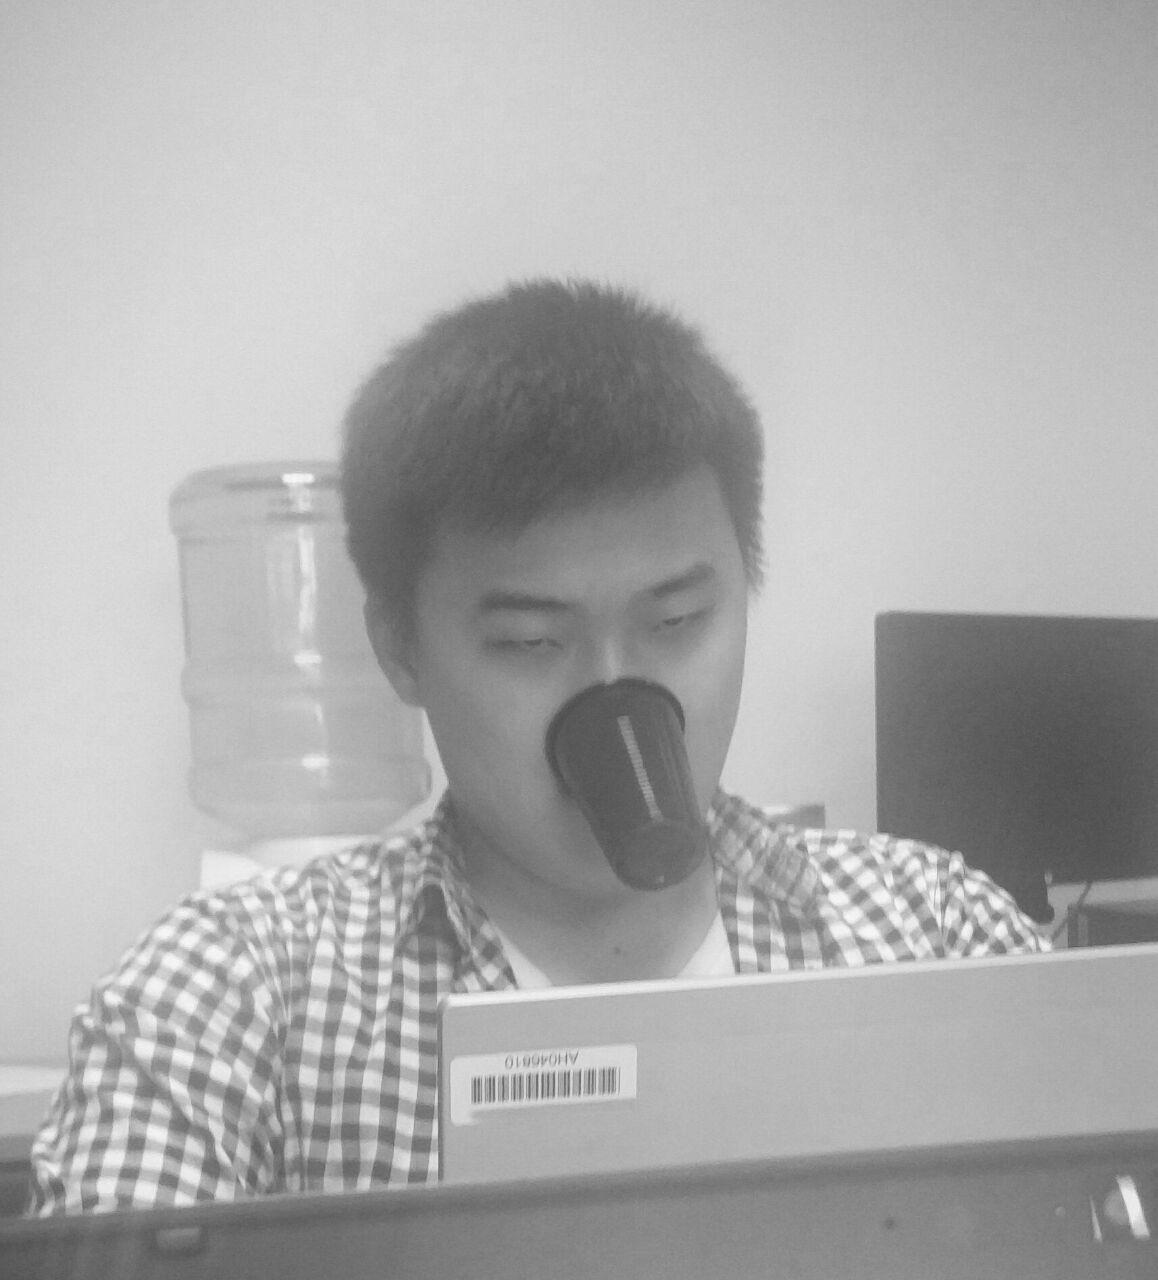
\includegraphics[width=0.80\textwidth]{grey}
	\caption{Черно-белое изображение}
	\label{pic:grey}
\end{figure}

\subsection{Оператор Собеля}

Применим к изображению оператор Собеля (\vref{pic:sobel}).

\begin{figure}[H]
	\centering
	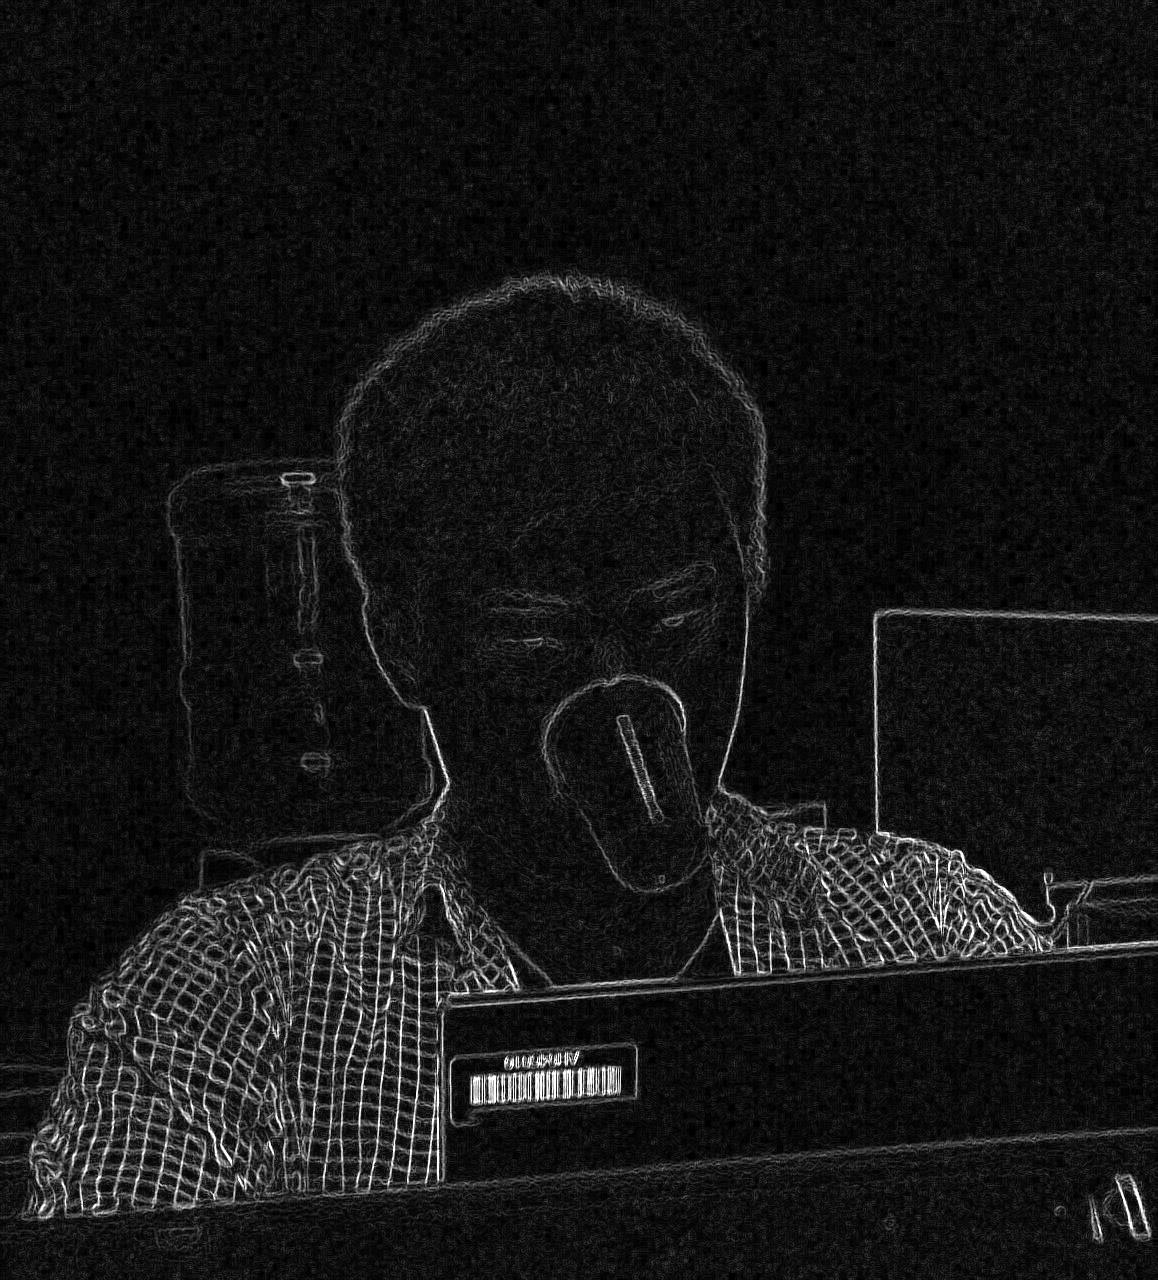
\includegraphics[width=0.80\textwidth]{sobel}
	\caption{Оператор свертки Собеля}
	\label{pic:sobel}
\end{figure}

\subsection{Оператор Превитта}

Применим к изображению оператор Превитта (\vref{pic:prewitt}).

\begin{figure}[H]
	\centering
	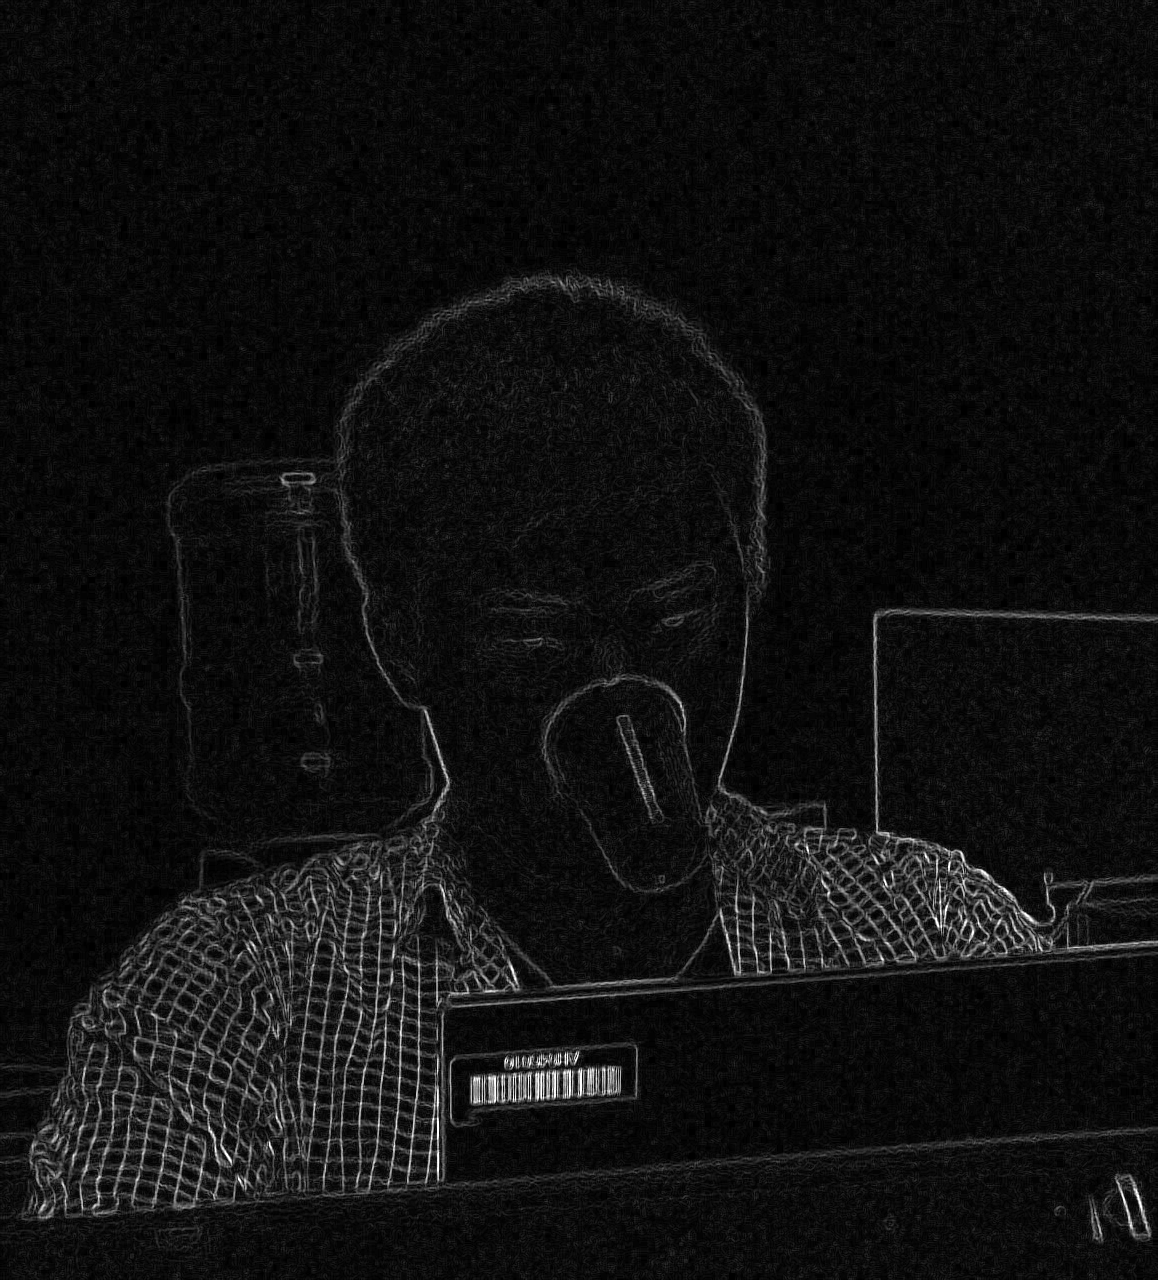
\includegraphics[width=0.80\textwidth]{prewitt}
	\caption{Оператор свертки Превитта}
	\label{pic:prewitt}
\end{figure}

\subsection{Оператор Робертса}

Применим к изображению оператор Робертса (\vref{pic:roberts}).

\begin{figure}[H]
	\centering
	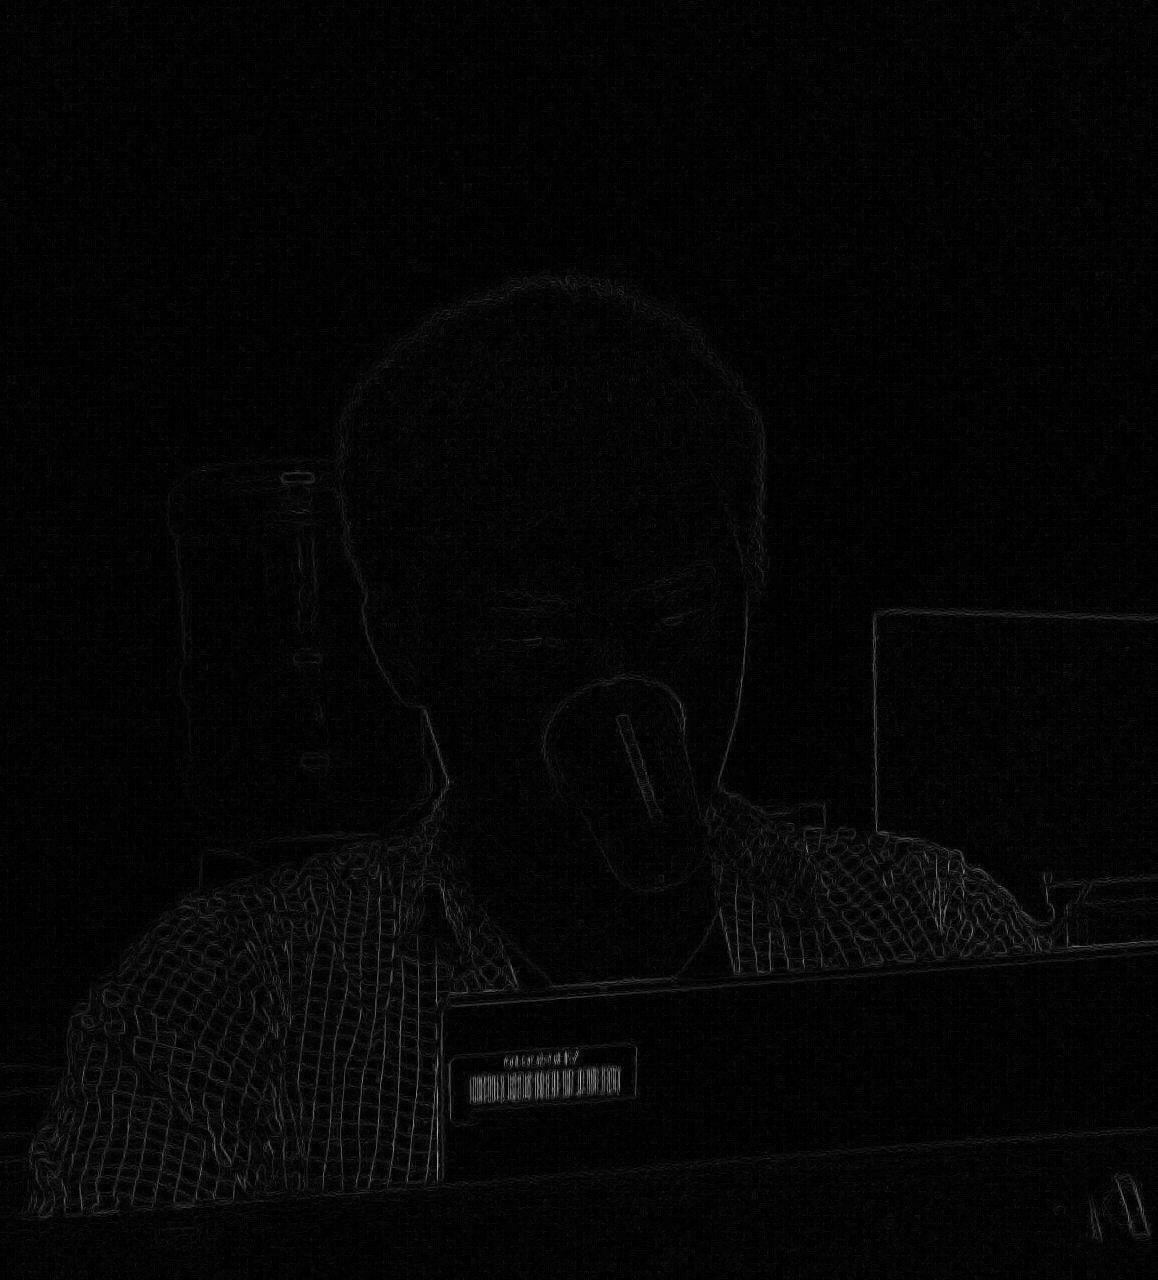
\includegraphics[width=0.80\textwidth]{roberts}
	\caption{Оператор свертки Робертса}
	\label{pic:roberts}
\end{figure}

\section{Выводы}

В ходе выполнения данной лабораторной работы к изображению были применены три оператора выделения контуров.

Оператор Собеля отличается самыми толстыми контурами, позволяя очень ярко и контрастно выделять линии. При этом выделение мелких объектов в данном операторе работает очень плохо. Лучше всего данный оператор проявляет себя при выделении вертикальных и диагональных линий.

Оператор Превитта также хорошо справляется с вертикальными и диагональными линиями. При обработке вертикальных линий данный оператор позволяет увидеть их даже в местах с большим количеством шумов. Однако мелкие детали и объекты выделяются также не очень хорошо, из-за они превращаются в шум. 

Оператор Робертса, по сравнению с операторами Превитта и Собеля, отличается наименее тонким выделением границ, но в то же время, он более четко выделяет мелкие, сгруппированные объекты и диагональные линии.